\cleardoublepage %poner esta linea al inicio de cada capitulo
\chapter{Banco de Pruebas}
As it is shown in \autoref{fig:Robotino}.
\begin{figure}[h]
    \centering
    \resizebox*{5cm}{!}{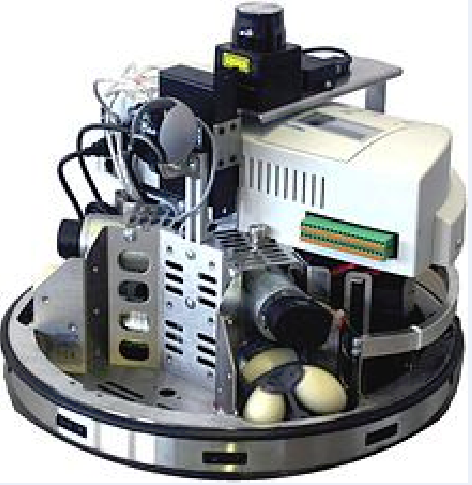
\includegraphics{Figs/robotino.PNG}}
    \caption{Robotino}
    \label{fig:Robotino}
\end{figure}


Texto dentro del capítulo 2 ...cap\'itulo 2....


\section{Descripci\'on general}
Descripci\'on, todas las conexiones, drivers, encoders, tarjetas adq, toolbox realtime, config de simulink para realtime, grabar datos, rangos de cada variable, salidas pwm, salidas AO, entradas encoder, entradas/salidas digitales, config de ganancias y par\'ametros de todo....

\section{Mecanismo de Backlash}

\subsection{Dise\~no y construcci\'on}
La validación experimental es

\subsection{Modelado}


\subsection{Validaci\'on experimental}


\section{Modelado y validaci\'on del sistema mecatr\'onico}
Influye din\'amica del motor, fricciones de coulomb y est\'aticas, backlash, cambio de inercia y perturbaci\'on externa (freno)...an\'alisis de cotas en las no linealidades y en las perturbaciones externas. Debe haber simulaciones, experimentos para hallar cada par\'ametro y validaci\'on del sistema completo....Al final debe haber un modelo no lineal con incertidumbres caracterizadas que tenga dos entradas: ciclo \'util al motor y perturbaci\'on externa(freno), y dos salidas: posici\'on angular antes del backlash y posici\'on angular despu\'es del backlash... y pues ese modelo validado con experimentos aplicando se\~nal a ambas entradas y comparando las salidas